\chapter{光传输特性的模拟及计算}
数值模拟是研究气动光学效应的有效手段,相对实验研究而言,采用数值模拟方法可以更加全面地控制模拟条件并且能够对模拟过程多次重复,给出正确的初始条件就可以得到精确且定量的结果,本章对于光学传输部分的数值计算均采用Mathematica数学计算工具。光场的重要参数~--~折射率能够通过流场密度转换得到,通过折射率的分布、起伏情况结合线性光学及统计光学等计算方法,就能描述出光束的传播过程。
\section{流场密度到折射率的转换及计算}
通过波动方程\eqref{eq:guangbodong}可以看出,光波的传输主要收到折射率分布的影响,由此可知研究光传输特性时,首先应该求流场的解折射率。气体的折射率往往受到流场的压力、密度及温度等状态参数影响,而一般情况下,气体的折射率大小主要取决于气体的密度,通过洛伦兹-洛伦茨公式,可以得到流场的密度与折射率之间的直接关系\cite{max2001},如式\eqref{eq:luolunzi}:
\begin{equation}
\Big(\frac{n^2-1}{n^2+2}\Big)\cdot\frac{1}{\rho}=\frac{2}{3}K_{GD}
\label{eq:luolunzi}
\end{equation}
式中,$K_{GD}$为气体密度到折射率的转换系数,称为$G-D$系数,$n$为气体折射率, $\rho$为气体密度,由于大气密度略大于1,可以进行简单的近似,即$n^2-1\approx2(n-1),n^2+1\approx3$,可以得到简单的密度到折射率的转换关系\cite{yxl2003qdgxyl}:
\begin{equation}
n=1+K_{GD}\cdot\rho
\label{eq:gdgongshi}
\end{equation}

标准空气的$G-D$系数与波长存在一定的函数关系,并且在红外区域,该系数基本保持不变,表达式可以近似为式:
\begin{equation}
K_{GD}=2.23\times 10^{-4}(1+\frac{7.52\times 10^{-3}}{\lambda^2})
\end{equation}
式中,$\lambda$为波长,单位$(\mu\text{m})$,$K_{GD}$单位$(\text{cm}^3/\text{g})$。本文计算并列举了$0.2\sim0.9\mu\text{m}$波长对应的$G-D$系数,如表\ref{tab:gdxishu}。
\begin{table}[bthp]
\caption{$G-D$系数表}
\label{tab:gdxishu}
\centering
\begin{tabular}{|c|c|c|c|}
\hline
波长($\mu \text{m}$)&$G-D$系数$(\text{cm}^3/\text{g})$&波长($\mu \text{m}$)&$G-D$系数$(\text{cm}^3/\text{g})$\\
\hline
0.2&0.2642&0.6&0.2220\\\hline
0.3&0.2385&0.7&0.2205\\\hline
0.4&0.2281&0.8&0.2201\\\hline
0.5&0.2236&0.9&0.2198\\\hline
\end{tabular}
\end{table}

通过折射率与密度的对应转换关系,就可以求出相应的折射率分布。本文以第三章中通过计算流体力学软件模拟得到的机载凸台周围流场为例,选取运行速度为2倍音速情况,为了比较清晰地展现高速流场的分布情况,可以以凸台光学窗口为基准截面,选取窗口周围约0.75m$\times$1.4m范围的长方形区域,利用公式\eqref{eq:gdgongshi}得到从密度到折射率的转换,如图\ref{fig:midudaozheshelv}。
\begin{figure}[bhtp]
\centering
\subcaptionbox{截面区域密度}{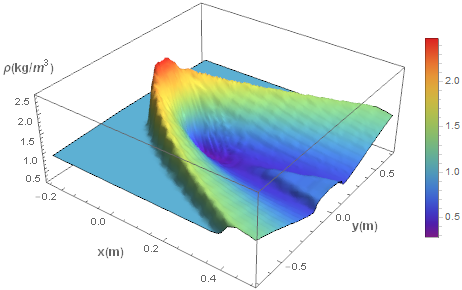
\includegraphics[width=0.49\linewidth]{tutaijiemianmidu.png}}
\subcaptionbox{截面区域折射率}{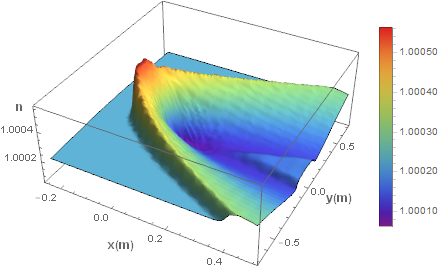
\includegraphics[width=0.49\linewidth]{tutaijiemianzheshelv.png}}
\caption{凸台周围截面密度及折射率分布情况}
\label{fig:midudaozheshelv}
\end{figure}

在图\ref{fig:midudaozheshelv}中,可以明确地看到剪切层的存在,并且剪切层中的密度及折射率比远处流场高,而在凸台正上方近壁面处,流场密度及折射率明显减弱,且低于平均值。根据第三章的分析,这是由于凸台顶部为半球,正中间处于最高位置,紧接着凸台结构呈下降趋势,这种结构的改变引起了高速流场的变化,在距离凸台底部高度为0.2m,以凸台中心为几何中心,尺寸为0.75m$\times$1.4m的长方形截面上,折射率波动位于1.00006$\sim$1.00056之间,正是这种不规则的折射率脉动起伏导致了光束传输过程中的畸变存在。
\section{光束的数学表达及衍射分析}
流场对光束的传输影响一般通过衍射理论来分析,利用流场密度转换成折射率后,通过折射率的脉动等参数计算出相位畸变、光学传递函数等,能够根据衍射图来评价流场对光传输的影响。
\subsection{基模高斯光束的传输特性}
通常情况下,光学设备接受、发射的激光光束均满足高斯分布,在所有可能的激光光束中基模高斯光束最具有典型性,它是一种具有特殊传输性质的高斯球面波,在研究中具有非常重要的作用,基模高斯光束的振幅表达式为\eqref{eq:gaosiguangshu}。
\begin{equation}
U(x,y,z)=\frac{A_0}{\omega(z)}\exp\big[\frac{-(x^2+y^2)}{\omega^2(z)}\big]\times\exp\big\{-ik\big[\frac{x^2+y^2}{2R(z)}+z\big]+i\varphi(z)\big\}
\label{eq:gaosiguangshu}
\end{equation}
式中,$z$为传输距离,$z$处光斑半径$\omega(z)=\omega_0\sqrt{1+(z/f)^2}=\omega_0\sqrt{1+[(\lambda z)/(\pi\omega_0^2)]^2}$,等相面曲率半径$R(z)=z[1+(f/z)^2]$,束腰半径$\omega_0=\sqrt{(\lambda f)/\pi}$,共焦参量$f=(\pi\omega_0^2)/\lambda$。

由式\eqref{eq:gaosiguangshu}可知,高斯光束的沿既定方向传播时会有一个特定的发散角,发散角与束腰半径成反比,而与波长成正比关系,束腰半径越小,它的光斑扩散越快。通过计算式,只要知道激光的波长,给定束腰半径,就可以知道在传输路径上每个截面上的光波表达式,从而知道光强分布。假设光斑的光强$I(x,y,z)$分布与振幅的模的平方相等,则可以令光强表示为\eqref{eq:guangqiang}。
\begin{equation}
\begin{aligned}
I(x,y,z)&=\big|U(x,y,z)\big|^2=U(x,y,z)\cdot U^*(x,y,z)\\
&=\frac{A_0^2}{\omega^2(z)}\exp\big[\frac{-2(x^2+y^2)}{\omega^2(z)}\big]
\end{aligned}
\label{eq:guangqiang}
\end{equation}

本文采用的基模高斯光束的束腰半径为$w_0=0.5$mm,波长为$\lambda=0.6328\mu$m的基模高斯光束,如图\ref{fig:gaussianbeam},为了方便计算,在取高斯光束时,对其进行了归一化处理,使其光强在$0\sim 1$之间。
\begin{figure}[bhp]
\centering
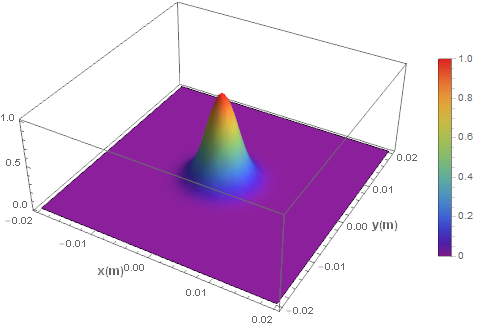
\includegraphics[width=0.45\linewidth]{gaussianbeam.png}
%\includegraphics[width=0.3\linewidth]{gaussianhuidu.png}
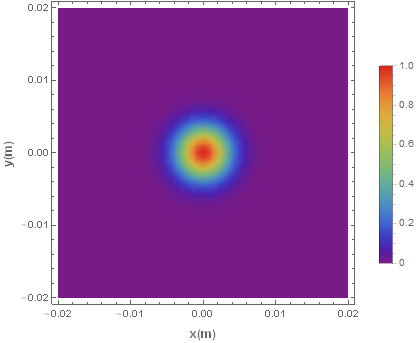
\includegraphics[width=0.45\linewidth]{gaussianbeamz=0.png}
\caption{束腰半径0.5mm的基模高斯光束}
\label{fig:gaussianbeam}
\end{figure}

对公式\eqref{eq:guangqiang}进行积分,同时将直角坐标系变换为极坐标系:$x=\omega(z)/\sqrt{2}\cdot\rho\sin\theta,y=\omega(z)/\sqrt{2}\cdot\rho\cos\theta$,能够得到z平面的光强:
\begin{equation}
\int_{-\infty}^{\infty}\int_{-\infty}^{\infty}I(x,y,z)\text{d}x\text{d}y=2A_0^2\int_0^{2\pi}\text{d}\theta\int_0^\infty\exp(-\rho^2)\rho\text{d}\rho=2\pi A_0^2
\end{equation}
式中,$A_0$为振幅,因此如果知道激光发射功率$P$,通过该式就能计算出高斯光束初平面的振幅,$A_0=\sqrt{P/2\pi}$。

事实上,在激光穿过流场时,会有能量的交换,激光对气体进行局部的加热从而损失一定的能量,如果用能量损耗系数$\beta$表示激光每传输一个单位的距离时相对损耗的功率,那么通过损耗系数就能够知道气体的升温率:
\begin{equation}
O(x,y,z)=\beta\cdot I(x,y,z)
\end{equation}
式中,$I(x,y,z)$表示空间上$(x,y,z)$点处的光强。

在通常情况下,谐振腔发出激光的振幅在横截面上的分布大多数呈现高斯函数的分布形式,而基模高斯光束在其中最具典型性,因此基模高斯光束的传输特性研究对于了解光学窗口处激光信号的接收发射具有重要意义。
\subsection{光波衍射的数值计算}
当光波经过小孔后,它的传输并不会按照线性光学理论所描述的会继续沿直线传播,而是会发生衍射现象,形成中心明亮的明暗相间的衍射圆环。一般衍射计量是利用夫琅禾费衍射作为依据的,夫琅禾费衍射又可以称作远场衍射,当平行光射入小孔时,在不同的传输距离上会出现不同的衍射光斑,光斑中心最亮,以第一圈暗环为分界线。中央的光斑强度占总强度的84\%左右,可以把这个中央亮斑称作爱里斑。当传输距离足够远时,光斑趋于稳定,随着距离的增加仅仅改变光斑半径,而衍射图样不发生变化,把这种衍射称为夫琅禾费衍射或远场衍射。

在第四章中经过流场作用后的夫琅禾费衍射可以由公式\eqref{eq:fraunhofer}表示,如果假设圆形小孔的直径为D,小孔的光学传递函数$OTF_D(x,y)$可以通过公式\eqref{eq:xiaokongguangchuandi}表示,点扩散函数可以表示为公式\eqref{eq:xiaokongdiankuosan}。
\begin{align}
OTF_D(x,y)&=\frac{2}{\pi}\Bigg[cos^{-1}\Big(\frac{\sqrt{x^2+y^2}}{D}\Big)-\frac{\sqrt{x^2+y^2}}{D}\sqrt{1-\Big(\frac{\sqrt{x^2+y^2}}{D}\Big)^2}\Bigg]
\label{eq:xiaokongguangchuandi}\\
PSF_D(x,y)&=\Bigg[2\cdot\frac{J_1\big[kD\sqrt{x^2+y^2}/(2L)\big]}{kD\sqrt{x^2+y^2}/(2L)}\Bigg]^2
\label{eq:xiaokongdiankuosan}
\end{align}
式中,由于小孔孔径外光学传递函数为零,因此需满足$\sqrt{x^2+y^2}\leq D/2$的条件。

通过公式\eqref{eq:xiaokongguangchuandi}、\eqref{eq:xiaokongdiankuosan}可以得到平面光波经过小孔衍射后的衍射光斑,如图\ref{fig:xiaokong}。事实上由于夫琅禾费衍射需要成立条件苛刻,需要在很远才能观测到衍射图案,实验条件难以达到,因此可以在小孔后面紧贴着放置一块焦距为d的透镜,将光波汇集到焦平面上,这样保证成像图案不变,仅改变了大小比例,由于一般仅需要观测夫琅禾费衍射的光斑分布,因此这种方法非常有效。
\begin{figure}[bhtp]
\centering
\subcaptionbox{直径为0.1cm的圆孔光学传递函数}{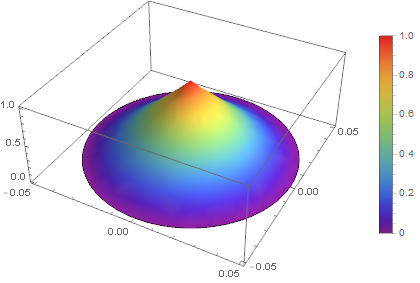
\includegraphics[width=0.45\linewidth]{xiaokongguangchuandi.png}}
\subcaptionbox{传输距离4km的夫琅禾费衍射}{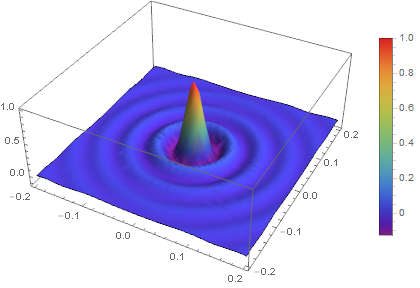
\includegraphics[width=0.45\linewidth]{fraunhofer.png}}
\caption{衍射孔光传递函数及夫琅禾费衍射}
\label{fig:xiaokong}
\end{figure}

由于实际流场结构的复杂性,通过上述衍射积分方法求解光学传递函数从而计算光场分布难以实现,通常情况下需要采用数值计算,为了在保证计算精度的同时简化计算量,可以采用稳相法来进行优化的数值计算,即采用渐进公式,利用代数运算替代复杂的积分公式。
\section{凸台光学窗口周围流场引起的光束畸变分析}
光束在湍流流场传播过程中的相位畸变主要是由于折射率脉动导致的,而折射率的脉动又由流场密度脉动引起,因此可以通过流场的密度脉动来求解相位畸变。通过$G-D$系数可以将密度与折射率联系起来,因此知道了流场密度,同时通过光线追迹法知道了光传输路径,就可以计算出光束的相位畸变。
\subsection{基于CFD网格的波面畸变计算}
由于在划分流场计算网格时,对边界层进行了加密处理,如图\ref{fig:tutaijiemianwangge}所示,因此从光学窗口到远离壁面之间的计算网格并非同样大小,越靠近光学窗口处网格越密,网格边长越小,本文以光学窗口中心为三维直角坐标系原点,形成$x-y$平面平行于窗口,$z$轴垂直于窗口平面的坐标系。

假设第$i$层网格上表面距离原点$l_i$,第$i+1$层网格上表面距离原点$l_{i+1}$,光线入射到第$i+1$层的入射角为$\theta_i$,根据直角三角形勾股定理以及直角余弦定理,可以近似地计算出光线在第$i$层网格中的实际传输距离$\Delta l_i$为$(|l_{i+1}-l_i|/\cos\theta_i)$
,每个网格中的折射率可以看作是前后表面折射率的算数平均即$(n_{i+1}+n_i)/2$,折射率差$\Delta n_i$可以定为$(n_{i+1}+n_i)/2-\bar{n}$,那么可以知道第$i$个网格中的光程差OPD应该为$\Delta l_i\cdot\Delta n_i$,对光束传播方向上的每一个网格中的光程差累加后就可以得到该条光线经过流场后的总的光程差:
\begin{equation}
\Delta L=\sum\limits_{i=1}^{\rm N}\frac{|l_{i+1}-l_i|}{\cos\theta_i}\cdot(\frac{n_{i+1}+n_i}{2}-\bar{n})
\label{eq:wanggegaungchengcha}
\end{equation}
式中,N为沿光传输方向的网格数量。

在计算光程差时,本文将网格沿光束传播方向分层,假定在同一层间传输方向不变,即如果光束在经过同一层不同网格时,仍保持传输方向,那么如果已知入射到第$i+1$层的入射角$\theta_i$,通过正弦定律可以得到第$i+2$层的入射角$\theta_{i+1}$,两者有如下关系:
\begin{equation}
(n_{i+1}+n_i)\cdot\sin\theta_i=(n_{i+2}+n_{i+1})\cdot\sin\theta_{i+1}
\label{eq:zhengxianjiao}
\end{equation}

通过式\eqref{eq:zhengxianjiao},给出初始入射角$\theta_0$就能经过计算得到光线入射到每一个网格面的入射角,将其反带入公式\eqref{eq:wanggegaungchengcha},进行离散的累加计算后,就能计算出每一条光线经过整个计算区域的光程差。
采用上述方法,对每一条光线进行追踪计算,得到了光学孔径上每一个入射到格点的光线光程差,通过对这些离散的光程差进行差值后,就能近似地得到时间平均的流场对光束在传播方向上的波面畸变情况。

通过第四章的理论分析,能够明确知道相位实际上是光程与波数的乘积,那么相位差就是光程差与波数的乘积,因此在给定波长的情况下,光波的光程差直接决定了光波相位畸变$\Delta \phi$的大小,如果入射光波波长为$\lambda$对应的光程差为$\Delta L$,那么光波的相位畸变可以写为如下表达式:
\begin{equation}
\Delta\phi=k\cdot\Delta L=\frac{2\pi}{\lambda}\cdot\Delta L
\label{eq:xiangweijibian}
\end{equation}

在基于CFD网格划分对光程差进行计算时,可以看出网格的划分情况对于计算至关重要,本文对机载光学凸台周围的网格按照流场流向划分,与Fluent的模拟结果较为契合,大大简化了基于直角三维坐标系的计算过程,对坐标系的建立能能够直接与网格走向一致。

以一倍音速以及两倍音速运行下的机载凸台光学设备周围流场为例,由于光学窗口大约位于凸台底部上方10cm左右,因此本文在凸台上方10cm处的近壁面取一个包含剪切层的流场,流场尺寸为长0.9m宽0.4m,高0.15m的长方体区域,查看不同速度下的波面畸变情况,图\ref{fig:zfangxiangguangchengcha}显示了不同速度下机载凸台光学窗口周围流场分布以及波面畸变情况,令x方向为飞行器前进方向。

\begin{figure}[bhtp]
\centering
\subcaptionbox{1Ma速度下流场底面及切面\label{fig:1matutaiqiemian}}{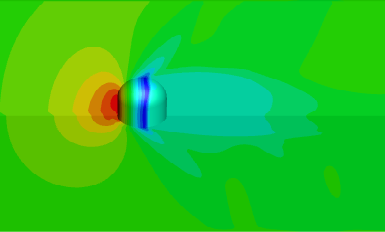
\includegraphics[width=0.48\linewidth]{1matutaicemian.PNG}}
\subcaptionbox{1Ma速度下光学窗口周围光程差\label{fig:tutaizhouweiguangchengcha1z}}{
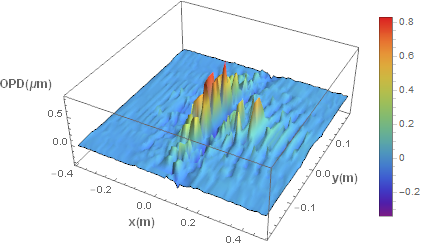
\includegraphics[width=0.48\linewidth]{tutaizhouweiguangchengcha1maz.png}}\\
\subcaptionbox{2Ma速度下流场底面及切面\label{fig:2matutaiqiemian}}{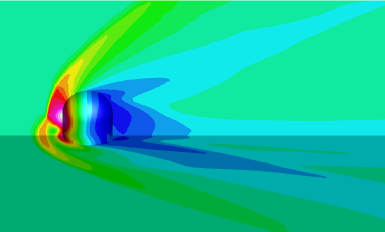
\includegraphics[width=0.48\linewidth]{2matutaicemian.PNG}}
\subcaptionbox{2Ma速度下光学窗口周围光程差\label{fig:tutaizhouweiguangchengcha2z}}{
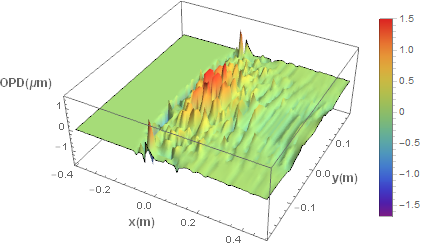
\includegraphics[width=0.48\linewidth]{tutaizhouweiguangchengcha2maz.png}}
\caption{不同速度下光束沿z方向传播的波面畸变}
\label{fig:zfangxiangguangchengcha}
\end{figure}

图\ref{fig:1matutaiqiemian}、\ref{fig:2matutaiqiemian}为通过计算流体力学软件模拟的两种不同速度下机载凸台底面以及中轴切面的流场密度分布情况,图\ref{fig:tutaizhouweiguangchengcha1z}、\ref{fig:tutaizhouweiguangchengcha2z}分别在一倍以及两倍音速下,光束沿z方向入射时,经过15cm厚的非均匀流场后在光学窗口处的波面畸变情况。可以发现当速度为1Ma时,沿z方向的光束光程差在$-0.3\mu\text{m}\sim0.8\mu\text{m}$之间波动,并且在凸台前方、周围近壁面及光学窗口后方的波面畸变较严重,而在2Ma运行速度下,光程差分布于$-1.6\mu\text{m}\sim1.5\mu\text{m}$之间,并且在凸台前方由于流场的压缩,光波仅在靠近壁面处产生畸变,随着速度的提升,波前畸变也会更加严重。

从图\ref{fig:tutaizhouweiguangchengcha1z}、\ref{fig:tutaizhouweiguangchengcha2z}能够发现在2Ma速度下光学窗口前方约12cm外的流场已经是均匀分布,这时光束在均匀流场中传输并不产生光程差,而1Ma下在更远处流场才呈现均匀性,因此在计算不同运行速度下飞行器的气动光学效应时,对于剪切层及湍流外边界的确定能够以此为参考。

由于图\ref{fig:zfangxiangguangchengcha}中计算了光束沿垂直于光学窗口方向入射进流场,经过15cm厚度的流场后的光程差,而在大多数情况下,探测光线一般比较靠近飞行器前进方向,即与光学窗口轴向成较大的角度入射进光学探测窗口,为此,可以对比不同角度的入射光束的波面畸变情况,如图\ref{fig:xgangxiangguangchengcha}所示。

\begin{figure}[bhtp]
\centering
\subcaptionbox{1Ma速度下光学窗口周围光程差\label{fig:tutaizhouweiguangchengcha1x}}{
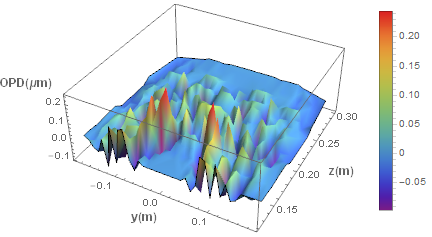
\includegraphics[width=0.48\linewidth]{tutaizhouweiguangchengcha1max.png}}
\subcaptionbox{2Ma速度下光学窗口周围光程差\label{fig:tutaizhouweiguangchengcha2x}}{
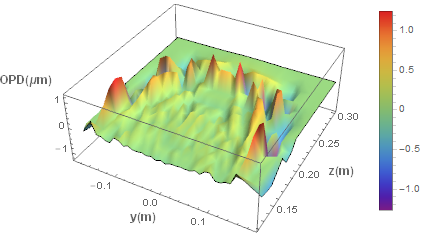
\includegraphics[width=0.48\linewidth]{tutaizhouweiguangchengcha2max.png}}
\caption{不同速度下沿前进方向产生的波面畸变}
\label{fig:xgangxiangguangchengcha}
\end{figure}

图\ref{fig:xgangxiangguangchengcha}分别显示了不同速度下,沿着飞行器前进方向传播的光束产生的光程差,由于沿前进方向的流场结构不同于垂直于前进方向的流场结构,根据图\ref{fig:midudaozheshelv}所示,在光学窗口前方约6cm处流场就已经可以看作为均匀远场状态,因此对于沿前进方向入射的光束,层流区域的选择需要进行相应的改变。

本文取机载凸台前方0至7cm厚度的长方体区域作为研究区域,对不同速度下的波面畸变进行计算,如图\ref{fig:tutaizhouweiguangchengcha1x}、\ref{fig:tutaizhouweiguangchengcha2x}所示,可以看出1Ma速度下光程差于-0.1$\mu{\rm m}\sim$0.25$\mu$m之间,2Ma下光程差位于-0.5到1.9$\mu$m之间,凸台周围的波面发生严重畸变。

对比图\ref{fig:zfangxiangguangchengcha}和图\ref{fig:xgangxiangguangchengcha}可以发现沿前进方向的光程差明显小于z方向的光程差,这和流场厚度有一定关系,同时也与流场在不同方向的结构不同有关,因此入射角度影响了高速飞行器周围流场的分析。

由公式\eqref{eq:xiangweijibian}可以看出相位差与光程差成正比关系,与波长成反比关系,由此推测,如果给定流场结构以及光波进入流场的方向,那么入射光波波长越大,流场引起的相位差越小,从而导致波前畸变越小,因此可以认为对于给定的流场,入射光波波长越大越好,但是由于激光能量与光波波长存在相反的关系,波长越长的光波能量越小,强度越弱,因此如何选定探测波长也成为比较关键的问题。
\subsection{基于斯特列尔比及光传递函数的光束质量分析}
斯特列尔比作为一个重要的气动光学评价指标,可以通过波面误差来计算,如公式\eqref{eq:strehljunfangcha}所示,而该公式中相位均方差的计算则相应地能够通过密度均方差来求解,从而计算出流场的斯特列尔比。

本节参考上节计算光束波面畸变的处理方法,主要基于网格格点数据离散的方式对斯特列尔比进行分层的叠加求解,合理地假设光学孔径尺寸远大于流场密度脉动尺寸,在此假设基础上求解出斯特列尔比及光学传递函数,分析光束经过流场前后的能量损失情况,并且给出流场对光学成像的影响分析。

\begin{figure}[bhtp]
\centering
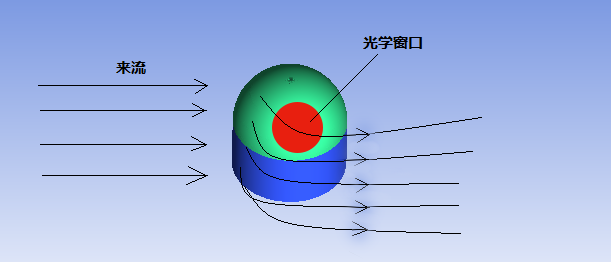
\includegraphics[width=0.9\linewidth]{tutaichuangkou.PNG}
\caption{机载凸台光学窗口示意图}
\label{fig:guangxuechaungkou}
\end{figure}

本文在对凸台光学窗口周围流场的气动光学效应进行计算时,根据凸台光学窗口距离底部的高度情况,选取了离凸台底部10cm高的光学探测窗口所处的流场区域,凸台光学窗口如图\ref{fig:guangxuechaungkou}所示。如果将流场厚度记为H,可以将非均匀流场划分为N个薄层,每层厚度为$h=$H/N,并且$h$大于湍流的涡旋尺度$l$,湍流的涡旋尺度根据在流场模拟中选用的模型的不同,也相应的有不同的经验估计方法,一般可以用$k-\varepsilon$和$k-\omega$模型的经验公式\eqref{eq:tuanliuchidu}。
\begin{equation}
\left\{
\begin{aligned}
&l=\frac{k^{3/2}}{\varepsilon}\cdot\frac{uL}{Re}~~~~~~~~&(k-\varepsilon\text{模型})\\
&l=\frac{k^{1/2}}{0.09\omega}\cdot\frac{uL}{Re}~~~~~~~~&(k-\omega\text{模型})
\end{aligned}
\right.
\label{eq:tuanliuchidu}
\end{equation}
式中,$u$为远场来流速度,$L$为飞行器结构长度,$Re$为雷诺数。

在计算密度均方差$\sigma_\rho^2$时,假定$\rho(x,y,z)$只取决于传输距离$z$而与孔径坐标$(x,y)$无关,那么就可以认为密度脉动均方差与$z$相关,记为$\sigma_\rho^2(z)$,同时记湍流在z方向的脉动尺度为$l_z(z)$,可以将相位均方差表示为如下公式所示:
\begin{equation}
\sigma_\phi^2\approx2K_{GD}^2\int_0^{\rm H}\sigma_\rho^2(z)l_z(z)\text{d}z
\end{equation}

在基于CFD软件模拟后的流场基础上计算时,可以通过网格格点将相位均方差公式离散,对传输方向每个网格面上的密度脉动均方差累加就能得到最终整个光瞳区域的密度脉动均方差,从而得到相位均方差:
\begin{equation}
\sigma_\phi^2\approx2K_{GD}^2\sum\limits_{i=1}^{N}\big[h_i\cdot\sigma_{\rho i}^2\cdot l_{zi}\big]
\label{eq:lisanxiangweimaidong}
\end{equation}
式中,$h_i$为沿传播方向第$i$层网格宽度,$\sigma_{\rho i}^2$表示第$i$层网格面上的密度脉动均方差,$l_{zi}$为z方向第$i$个网格处的脉动尺度。

利用离散点的相位均方差公式,结合大孔径近似下的斯特列尔比,见公式\eqref{eq:strehljunfangcha},就能够计算得到孔径为D的光学光口处斯特列尔比,也就是光束穿过流场后的产生像差后的中心光强与没有像差时中心光强的比值,这个比值显示了像点的分辨能力,从而可以对流场的气动光学效应做出相应的评估。

由于光束入射角度的不同,光束在流场中的传输路径也是不同的,这就导致光斑的光强分布随着入射角度的变化而变化,因此可以考虑几种不同的入射角,分别分析经过流场后的斯特列尔比。

本文以2Ma运行速度下的机载凸台为例,为了便于结合网格进行计算,在凸台光学窗口处截取了8$\times$8cm的方形光学孔径,根据第三章中的流场数值模拟结果,确定光学窗口处流场厚度为10cm,计算了垂直入射到光学孔径平面的光束产生的光程差,其等值图如图\ref{fig:chuangkoujibian}所示。

\begin{figure}[bhtp]
\begin{minipage}[b]{0.45\linewidth}
\centering
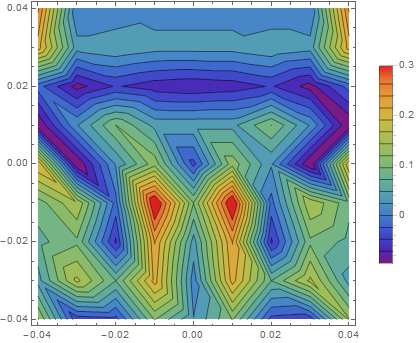
\includegraphics[width=\linewidth]{xiangweijibian.png}
\caption{光学窗口波面畸变($\mu$m)}
\label{fig:chuangkoujibian}
\end{minipage}
\begin{minipage}[b]{0.5\linewidth}
\centering
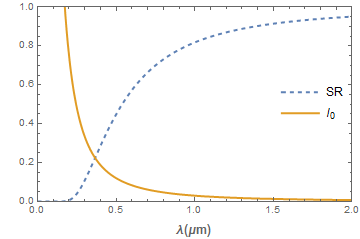
\includegraphics[width=\linewidth]{lixiangbizhi.png}
\caption{理想光强与斯特列尔比}
\label{fig:lixiangsite}
\end{minipage}
\end{figure}

采用公式\eqref{eq:lisanxiangweimaidong}的方法计算得到了相应的斯特列尔比约为25.37\%。为了进行对比,本文同时计算了光束在10$\textdegree$和20$\textdegree$两种不同角度下入射进光学窗口时的斯特列尔比分别为23.26\%和21.35\%,对比可以看出入射角度的变化一定程度上影响了光学成像质量,入射角越小,光束中心越亮,成像质量越好。


由于通过斯特列尔比表达式以及上述计算能够分析出在给定流场及入射角度情况下,斯特列尔比SR与光束波长平方的倒数成负指数关系($SR\propto\exp(-1/\lambda^2)$),而光强$I_0$与光束波长平方的倒数成正比关系($I_0\propto\dfrac{1}{\lambda^2}$),如图\ref{fig:lixiangsite}所示,图中的曲线仅表示光强与斯特列尔比的走势,实线为斯特列尔比随波长变化情况,虚线表示光强随波长变化情况,从对比图可以看出合适的探测波长选择也成为影响成像质量的重要因素,并且大量实验证明小于波长2$\mu$m的光波受到的气动光学效应影响比较严重。

通过第四章的理论分析,流场对光传输的作用能够分为平均流场部分和湍流随机脉动部分的综合作用,如果令平均流场以及脉动流场部分的光学传递函数分别为$f_{OTF1}(x,y),f_{OTF2}(x,y)$,那么两者对应相乘即可表示整个流场的光传递函数$f_{OTF}(x,y)=f_{OTF1}(x,y)\times f_{OTF2}(x,y)$,根据公式\eqref{eq:guangtonghanshu}定义光瞳函数$f(x,y)$为与光程差相关的函数,并且仅在光瞳孔径范围内存在,超出孔径范围则为零,那么通过光瞳函数自相关积与光传递函数存在等量关系,如公式\eqref{eq:pingjunguangchuandi}。
\begin{equation}
\left\{\begin{aligned}
&f_{OTF1}(x,y)=\frac{1}{S}\cdot f(x,y)*f(x,y)~~~~~~~~(x,y)\in {\rm A}\\
&f(x,y)=\exp(-i\Delta\phi)=\exp(-ik\Delta L)
\end{aligned}
\right.\label{eq:pingjunguangchuandi}
\end{equation}
式中,$S$是光学孔径的面积,A表示光学孔径区域,$\Delta L$表示光程差,$*$表示卷积。

而对于湍流随机脉动部分来说,光学传递函数主要与折射率的脉动起伏有一定的函数关系,
\begin{equation}
f_{OTF2}(x,y)=\exp\Big[-2k^2\int_0^H\overline{n'^2}(x,y,z)\cdot\big[l_{xyz}-\int_0^\infty C(x',y',z'){\rm d}z'\big]{\rm d}z\Big]
\label{eq:maidongguangchuandi}
\end{equation}
式中,本文选取指数模型的湍流相关系数$C(x',y',z')$,见公式\eqref{eq:zhishuxiangguanxishu},$\overline{n'^2}$为流场折射率脉动,可以通过流场密度分布求解,横向积分尺度$l_{xyz}$可以选择相应经验公式求解,本文采用公式\eqref{eq:tuanliuchidu}中的$k-\omega$模型的经验公式计算,经验公式中的流场基本参数主要由第三章中的凸台周围流场模拟部分给出。

因此,如果能够知道初始光束的表达式,通过公式\eqref{eq:pingjunguangchuandi}和公式\eqref{eq:maidongguangchuandi}得到整个流场的光学传递函数,就能给出经过流场后的光斑光强分布情况,如公式\eqref{eq:guangqiangfenbu}。
\begin{equation}
I(x',y')=\frac{1}{\lambda^2H^2}\iint\limits_{\rm A}I_0(x,y)f_{OTF}(x,y)\cdot\exp\big[\frac{2\pi}{\lambda H}(xx'+yy')\big]{\rm d}x{\rm d}y
\label{eq:gaungqiangfenbu}
\end{equation}
式中,由于传输距离较短,近似地将流场厚度$H$等价于光束实际路程,在基于网格计算时,需要将连续的积分公式转换为网格点的数值累加计算,如下所示:
\begin{equation}
I(x',y')=\sum\limits_{z=1}^{N}\frac{1}{\lambda^2h_z^2}\sum\limits_{i=1}^{N_x}\sum\limits_{j=1}^{N_y}I_0(x_i,y_j)f_{OTF}(x_i,y_j)\cdot\exp\big[\frac{2\pi}{\lambda h_z}(x_ix'+y_iy')\big]\cdot\Delta x\Delta y
\label{eq:gaungqiangfenbu1}
\end{equation}
式中,将流场分为N层,每层厚度为$h_z$,本文对近壁面处网格进行了加密,因此越靠近壁面,网格厚度$h_z$越小,每层网格在光学孔径上划分$N_x\times N_y$个小网格,网格边长分别为$\Delta x,\Delta y$。

本文将进入流场前的激光光束定义为束腰半径是1cm的基模高斯光束,截面光强分布满足高斯分布,如式\eqref{eq:guangqiang}所示,可以得到初平面的光强分布如图\ref{fig:chushigaosi}所示,采用式\eqref{eq:pingjunguangchuandi}、式\eqref{eq:maidongguangchuandi}以及式\eqref{eq:guangqiangfenbu}联立,代入公式\eqref{eq:gaungqiangfenbu1}后,通过基于网格格点的离散计算,同样对每段传输过程进行分层处理,并对结果进行归一化。计算区域为上述选定的厚度为10cm的流场区域,光束沿与光学窗口平面30\textdegree 角入射,光束偏移量通过上节光程差计算方法得到,通过平均及脉动流场叠加得到的光学传递函数$f_{OTF}$计算出了像平面的光强分布如图\ref{fig:jibiangaosi}所示。
\begin{figure}[bhtp]
\centering
\subcaptionbox{初平面高斯光束\label{fig:chushigaosi}}{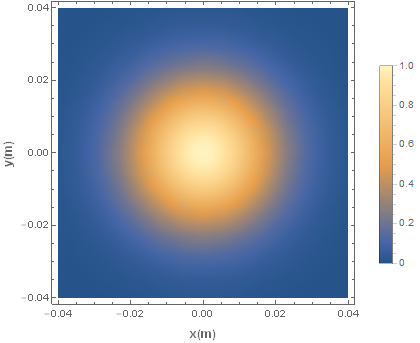
\includegraphics[width=0.45\linewidth]{yuanguangshu.png}}
\subcaptionbox{产生畸变后的高斯光束\label{fig:jibiangaosi}}{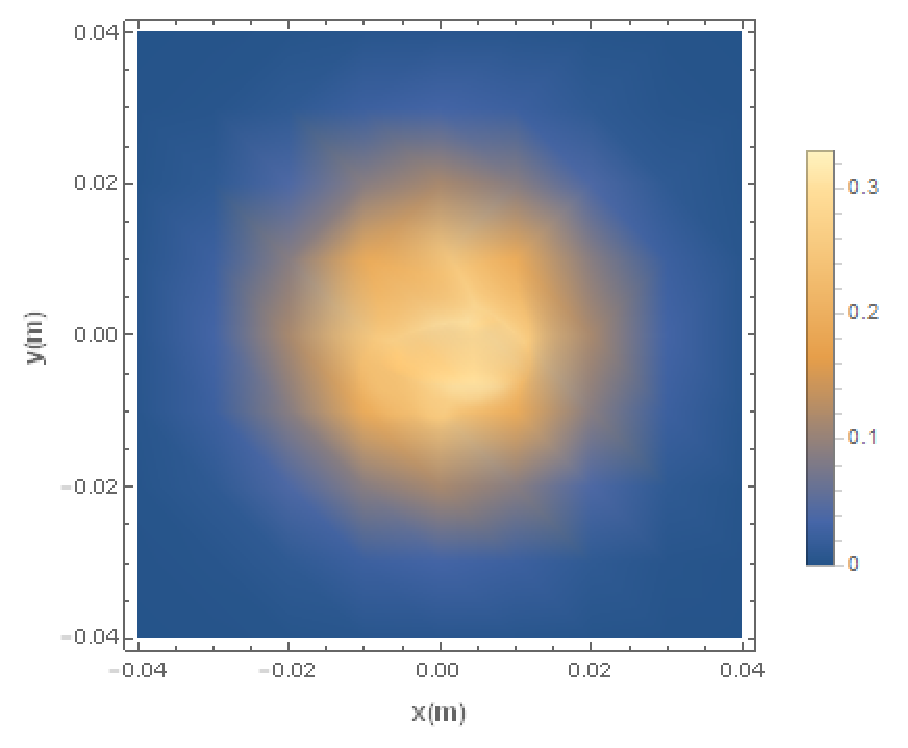
\includegraphics[width=0.45\linewidth]{pianyiguangshu.eps}}
\caption{高斯光束经过流场后的光场分布情况}
\end{figure}

通过对比光束经过凸台光学窗口周围流场前后的光斑情况,发现光斑中心亮度明显减弱,并且光场分布不再满足高斯分布,光强的分布受到整个流场在光学孔径上的光学传递函数影响,呈现不规则分布,光斑整体略有偏移,中心沿xy方向上的偏移距离为(0.022cm,-0.013cm),由此发现混合流场对于短距离成像的偏移作用很小,但是对于远距离传输情况而言,目标的成像及定位会因此产生较大的偏移。至此,通过斯特列尔比以及光学传递函数,较为明确地评价了光束经过流场的传输效应,为将来的光学校正提供了基础。
\section{本章小结}
本章基于Mathematica数据处理,通过Gladstone-Dale定律,完成了从流场参数到光学参数的转换,分析了2Ma运行速度下机载光学设备周围流场的折射率分布情况。对在实际应用中广泛使用的高斯光束的传播特性进行了研究并对其模拟成像,另外对圆形光学孔径的点扩散函数及光学传递函数进行了公式推导及计算,同时计算了远场夫琅禾费衍射的衍射图。最后对机载凸台周围的流场进一步分析,基于CFD计算网格的划分,讨论了流场对光波传输后的波面畸变的影响以及斯特列尔比的评价计算方法,对流场的气动光学效应进行了评估,计算了流场的光学传递函数,给出了高斯光束穿过流场后的光强分布情况。